% Template for PLoS

\documentclass[10pt]{article}

% amsmath package, useful for mathematical formulas
\usepackage{amsmath}
% amssymb package, useful for mathematical symbols
\usepackage{amssymb}

% hyperref package, useful for hyperlinks
\usepackage{hyperref}

% graphicx package, useful for including eps and pdf graphics
% include graphics with the command \includegraphics
\usepackage{graphicx}

% Sweave(-like)
\usepackage{fancyvrb}
\DefineVerbatimEnvironment{Sinput}{Verbatim}{fontshape=sl}
\DefineVerbatimEnvironment{Soutput}{Verbatim}{}
\DefineVerbatimEnvironment{Scode}{Verbatim}{fontshape=sl}
\newenvironment{Schunk}{}{}
\DefineVerbatimEnvironment{Code}{Verbatim}{}
\DefineVerbatimEnvironment{CodeInput}{Verbatim}{fontshape=sl}
\DefineVerbatimEnvironment{CodeOutput}{Verbatim}{}
\newenvironment{CodeChunk}{}{}

% cite package, to clean up citations in the main text. Do not remove.
\usepackage{cite}

\usepackage{color}

% Use doublespacing - comment out for single spacing
%\usepackage{setspace}
%\doublespacing


% Text layout
\topmargin 0.0cm
\oddsidemargin 0.5cm
\evensidemargin 0.5cm
\textwidth 16cm
\textheight 21cm

% Bold the 'Figure #' in the caption and separate it with a period
% Captions will be left justified
\usepackage[labelfont=bf,labelsep=period,justification=raggedright]{caption}

% Use the PLoS provided bibtex style
\bibliographystyle{plos}

% Remove brackets from numbering in List of References
\makeatletter
\renewcommand{\@biblabel}[1]{\quad#1.}
\makeatother


% Leave date blank
\date{}

\pagestyle{myheadings}
%% ** EDIT HERE **


%% ** EDIT HERE **
%% PLEASE INCLUDE ALL MACROS BELOW

%% END MACROS SECTION


\begin{document}

% Title must be 150 characters or less
\begin{flushleft}
{\Large
\textbf{Examining the explanatory model of the cultural continuity in Taiwan}
}
% Insert Author names, affiliations and corresponding author email.
\\
  Liying Wang\textsuperscript{1*}\\
\bf{1} Department of Anthropology, University of Washington,  Seattle,  Washington,  USA
\\

\textasteriskcentered{} E-mail:   \href{mailto:liying15@uw.edu}{\nolinkurl{liying15@uw.edu}}

\end{flushleft}

\subsubsection{Introduction}\label{introduction}

Data mining is a method to obtain the development of some topic over
time, and further examine the relevent articles. In this paper, I will
examine the term ``social inequality'' as a topic in archaeology by
using R. My potential questions for this quantitative research project
as following:

\begin{enumerate}
\def\labelenumi{\arabic{enumi}.}
\item
  What is the trend of research of social inequality in archaeology in
  the past decades? Is it popular in any particular time period?
\item
  How often social inequality relates to culture contact? Especially for
  European contact. Also, does any area show preference of such
  research, such as North America, Southeast Asia, Oceania, or Africa.
\item
  For the method, what is the relationship between the term
  ``inequality'' and other archaeological evidence, including burials,
  ceramics, post holes, or glass beads.
\end{enumerate}

In order to run the codes for my questions, I will use the two R
packages, JSTORs and devtools.

For the first question of the trend of social inequality, the plots show
that the topic of inequality becomes common after maybe 1992, and then
has became popular around 2006. The term ``social'' is commoner than the
term ``inequality''. I think the reason is that this term ``social'' is
too general. The third graph shows that social and inequality were
decussated together after 1978, but slightly goes down around 1986, and
then popular again from 1994. Based on the results, I can further
explore the exact articles with the word inequality.

The article with strongest correlation of the relationship of ``social''
and ``inequality'' as following: Sandra Montón Subías, 2007,
Interpreting Archaeological Continuities: An Approach to Transversal
Equality in the Argaric Bronze Age of South-East Iberia. World
Archaeology, Vol. 39, No. 2, The Archaeology of Equality, pp.~246-262.
Taylor \& Francis, Ltd

\begin{CodeChunk}

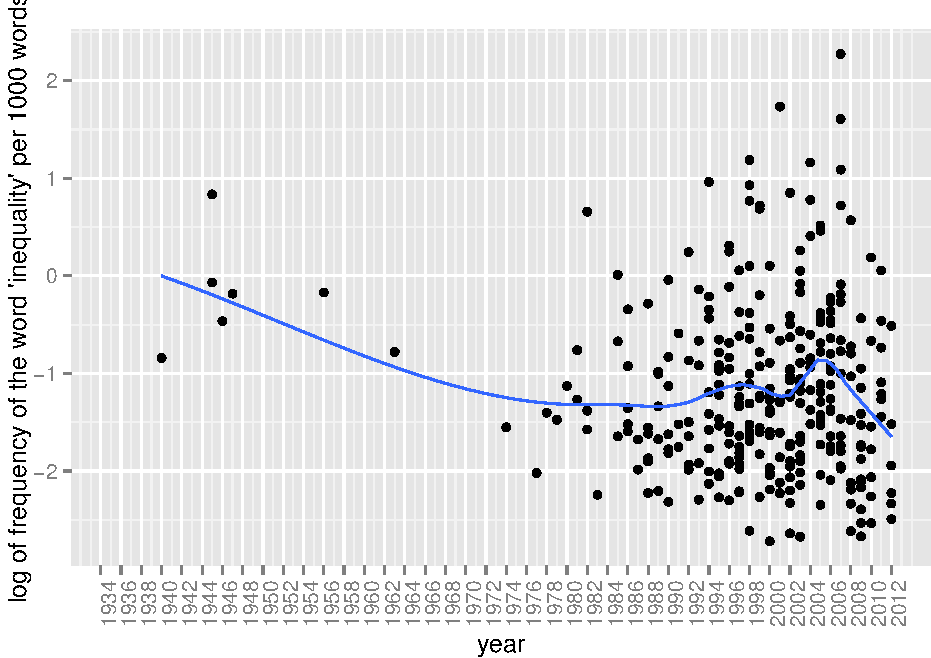
\includegraphics{509Assignment_files/figure-latex/onegram-1} \begin{CodeOutput}
Empty data.table (0 rows) of 3 cols: word_ratio,year,V2
\end{CodeOutput}

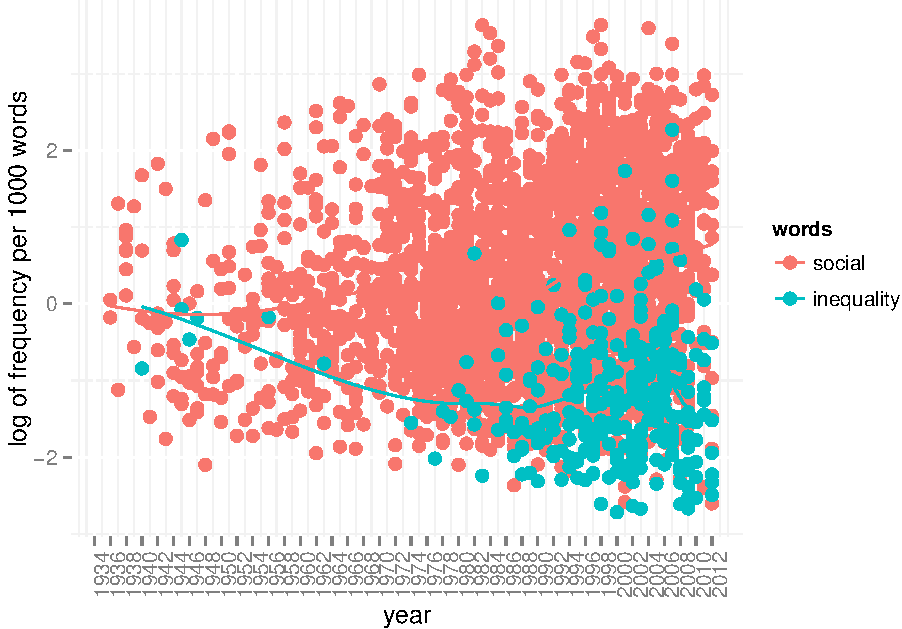
\includegraphics{509Assignment_files/figure-latex/onegram-2} \begin{CodeOutput}
   year variable    value             V2
1: 1998   social 38.05955 10.2307_125040
\end{CodeOutput}

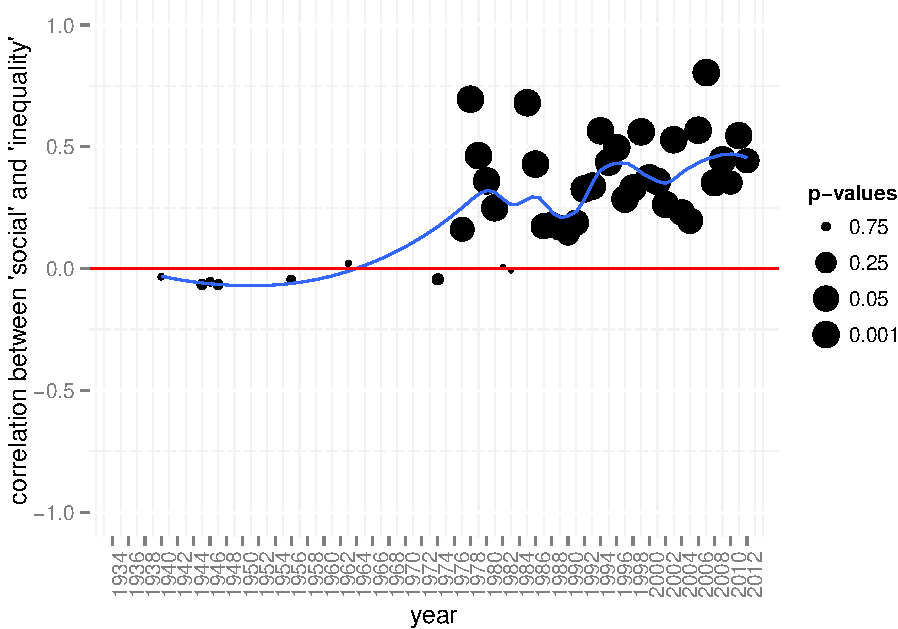
\includegraphics{509Assignment_files/figure-latex/onegram-3} \begin{CodeOutput}
   year variable    value               V2
1: 2007   social 29.81969 10.2307_40026656
\end{CodeOutput}
\end{CodeChunk}

If I use ``social inequality'' as a term, the plots shows that such
discussion only exists after 1978, becomes popular around 2000, and
slightly goes down at 2002. In archaeology, social inequality is one of
the indexes for social complexity. Therefore, I will also examine the
discussion of social complexity in order to have a general understanding
of such topic. The discussion of ``social complexity'' begins from 1947,
becomes popular at around 1978, slightly goes down at 1990 and 2006, and
then popular again at 2010. It seems like there is not big change in the
discussion of these two terms. If we examine these two terms over time,
the plot shows that they have different pattern of frequency. When
social inequality was frequently discusses, the frequency of social
complexity becomes lower. This might indicates the terms of social
inequality and social complexity might have some pattern of
relationship, which is to some extent mutually exclusive. Social
inequality could be viewed as more specific approach to social
complexity.

\begin{CodeChunk}

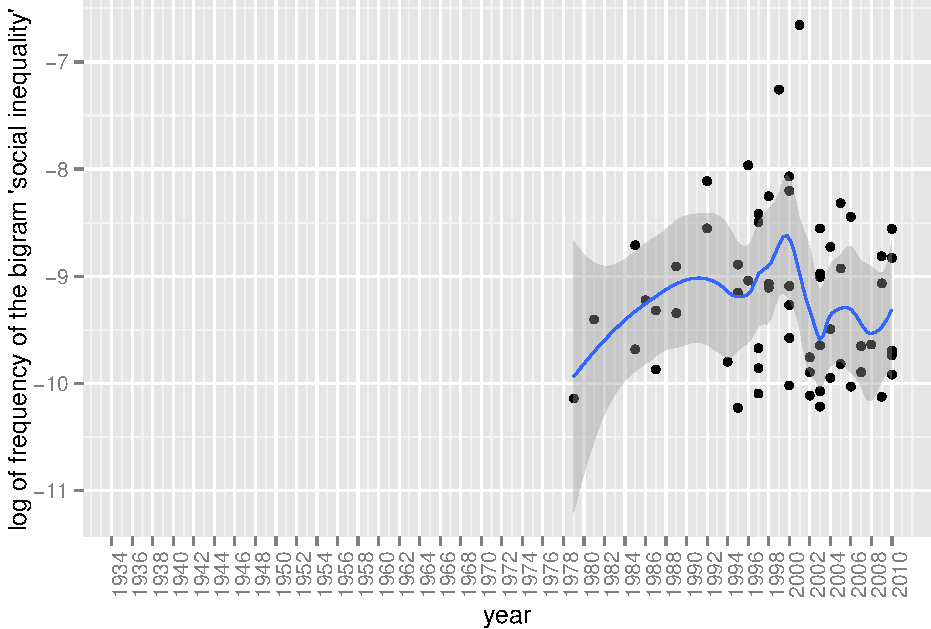
\includegraphics{509Assignment_files/figure-latex/bigrams1-1} \begin{CodeOutput}
   bigram_ratio year
1:  0.001287416 2001
\end{CodeOutput}

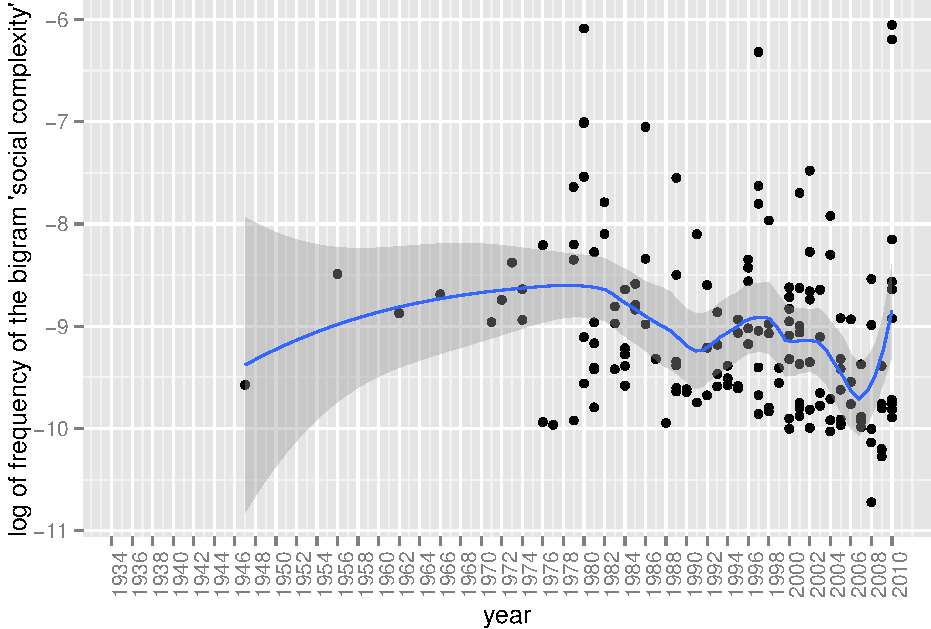
\includegraphics{509Assignment_files/figure-latex/bigrams1-2} \end{CodeChunk}

For the second question about the correlation between social inequality
and European contact, the plot of two terms shows that there is a
similar trend before 1994, but after 1994 there is no clear pattern
shows the relationship. When we further examine the correlation between
these two terms, the plot indicates that there is only an article shows
the relatively strong correlation at 1986. In addition to European
contact, I also examine the correlation between social inequality and
social complexity. The plot shows that they are strongly correlated at
1987, 1998, and 2007, which shows the periodic pattern of discussion.
This plot also explains the pattern in the former plot of word frequency
over time.

\begin{CodeChunk}

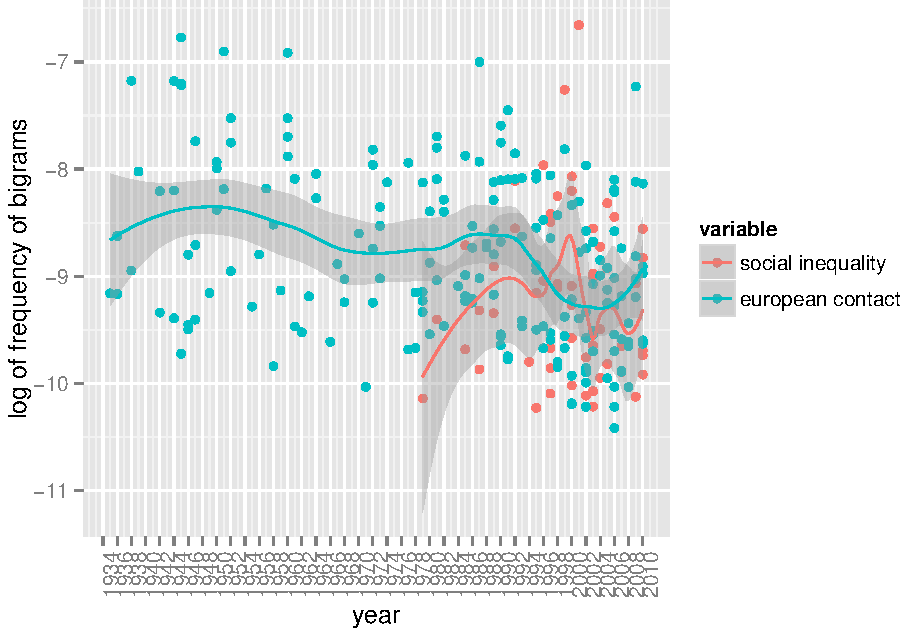
\includegraphics{509Assignment_files/figure-latex/bigrams-1} 
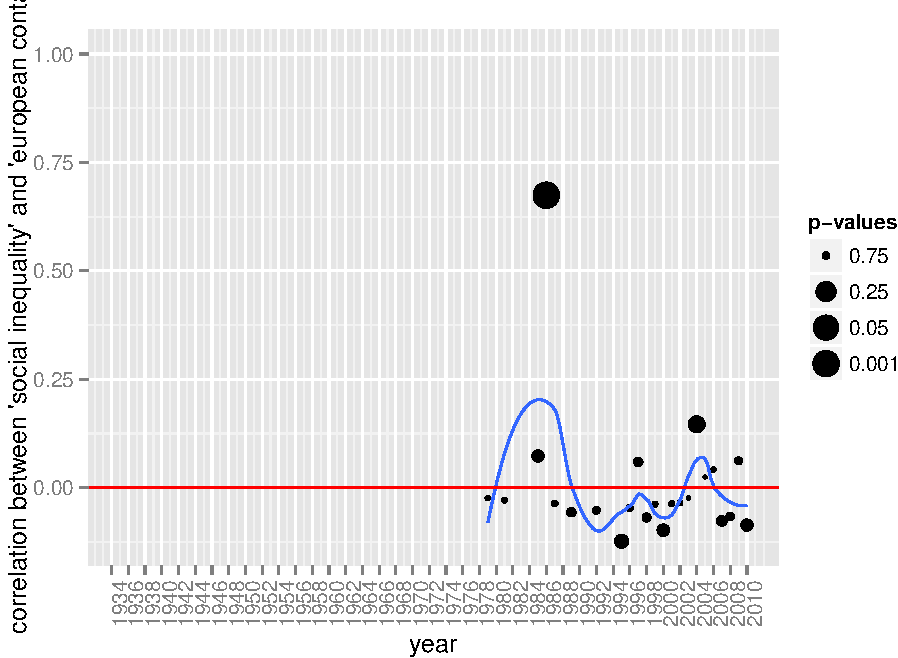
\includegraphics{509Assignment_files/figure-latex/bigrams-2} 
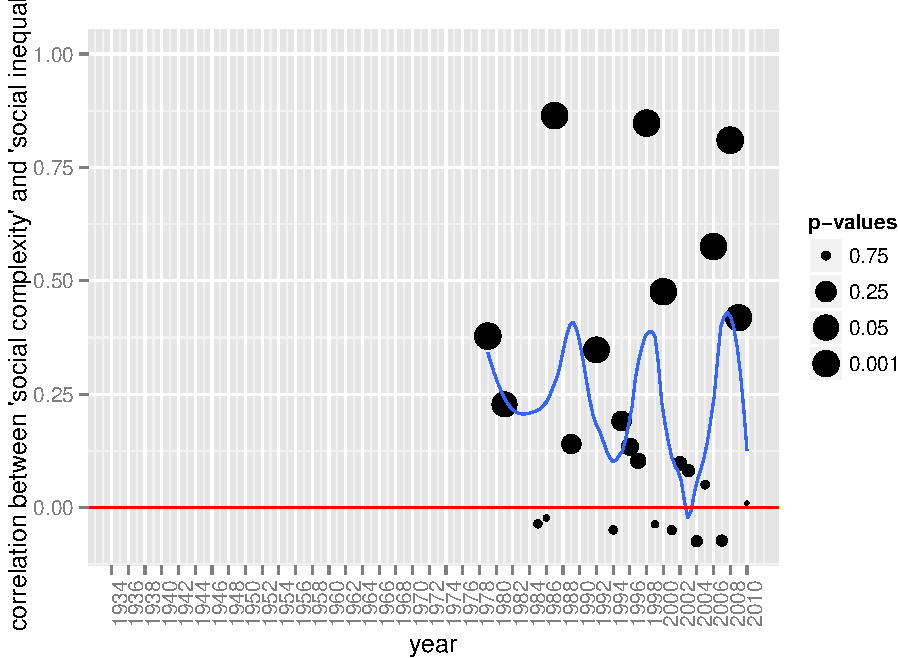
\includegraphics{509Assignment_files/figure-latex/bigrams-3} \end{CodeChunk}

I further examine the topic of inequality in terms of different areas,
such as Asia, Oceania, America, and Africa. The results show that in
Asia, most articles contain inequality exist after 1978, and the term
reached the highest frequency at 2004, but declined later at 2009. For
Oceania, the trend shows there are two periods with higher frequency,
which are 1996 and 2004. For America, there are more articles refer to
inequality, and this term was popular around 2005. The pattern of
frequency in Africa looks similar to the pattern in America, and also
shows the highest frequency at 2005. Although these four plots have
different trends of the frequency of inequality, it seems this term was
popular between 2004 and 2005 among these different areas.

For the third questions, these plots show the relationship between the
term `inequality' and other archaeological evidence, including beads,
burials, and pottery. For the beads, it indicates that a couple of
articles have strong positive correlation around 1990. In addition,
there is no much discussion until 1976. For the burials, it also shows
that the discussion of burial and inequality become common after the
publication of the article in 1976. Besides, is seems the articles could
be divided into two groups according to the extent of correlation. For
the pottery, there is no clear correlation until 2006. After 2006, some
articles show the positive correlation.

\begin{CodeChunk}

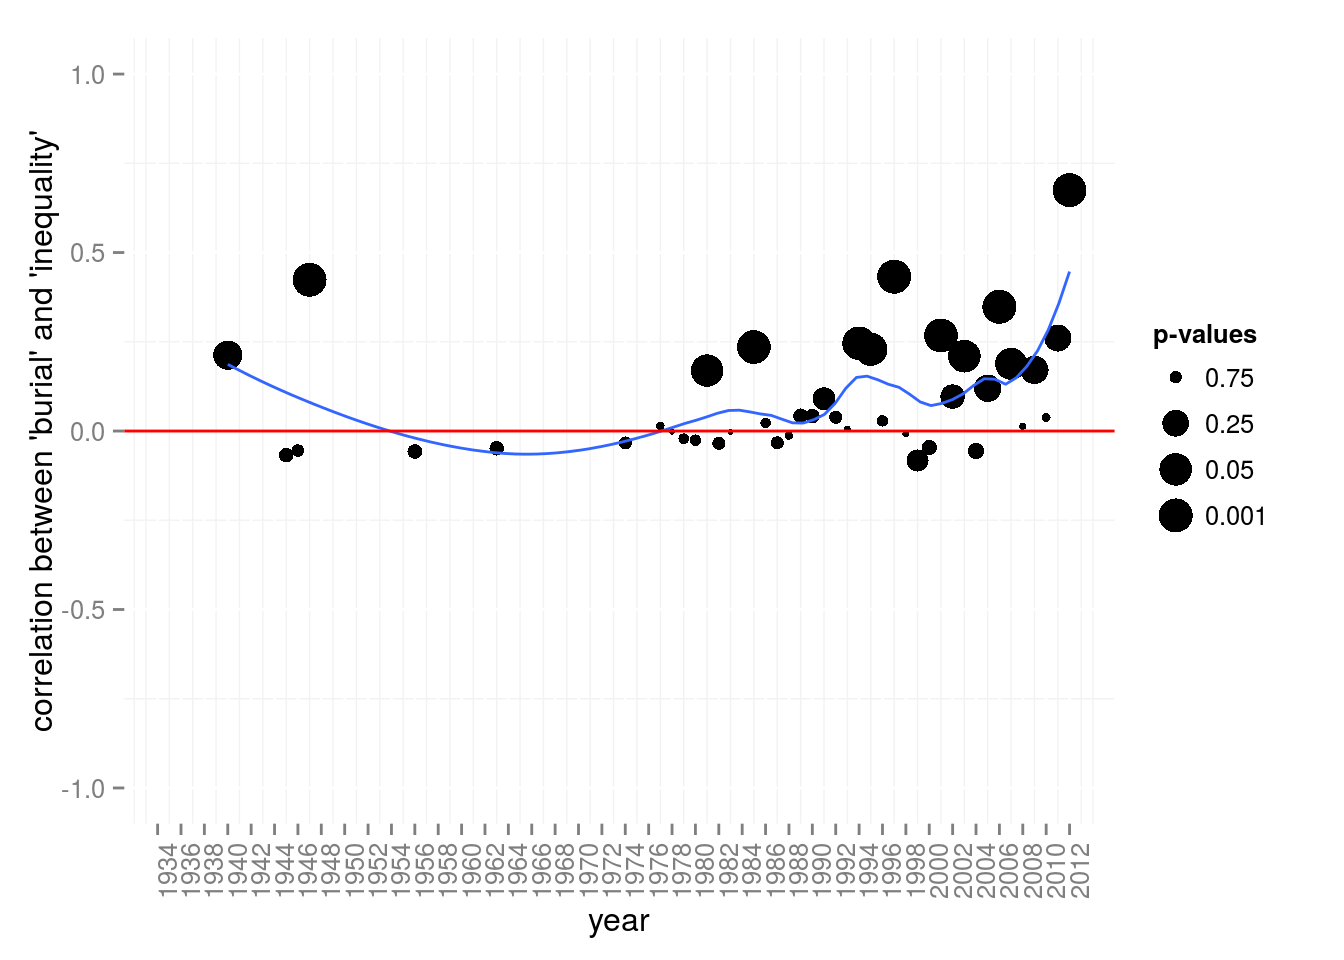
\includegraphics{509Assignment_files/figure-latex/onegram2-1} 
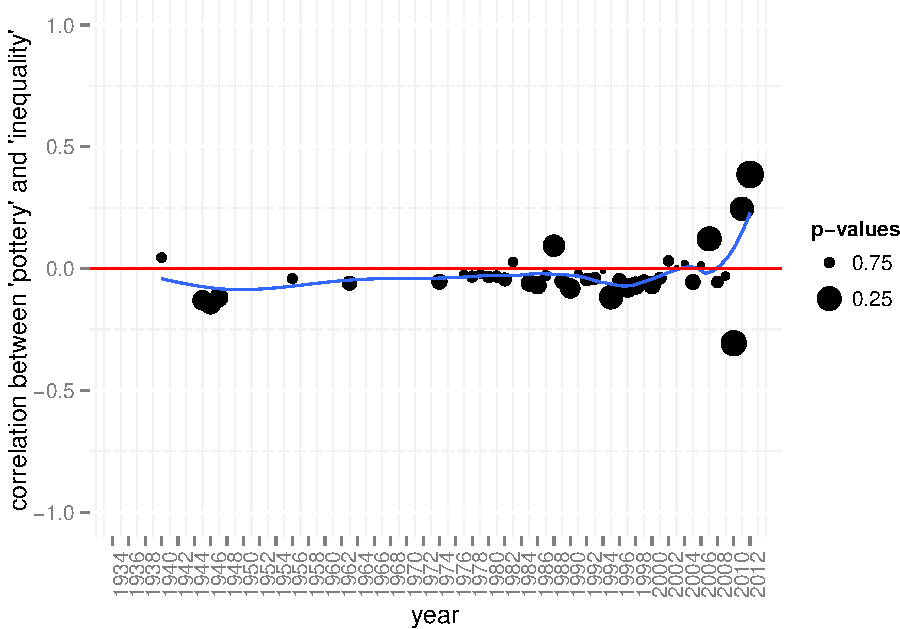
\includegraphics{509Assignment_files/figure-latex/onegram2-2} 
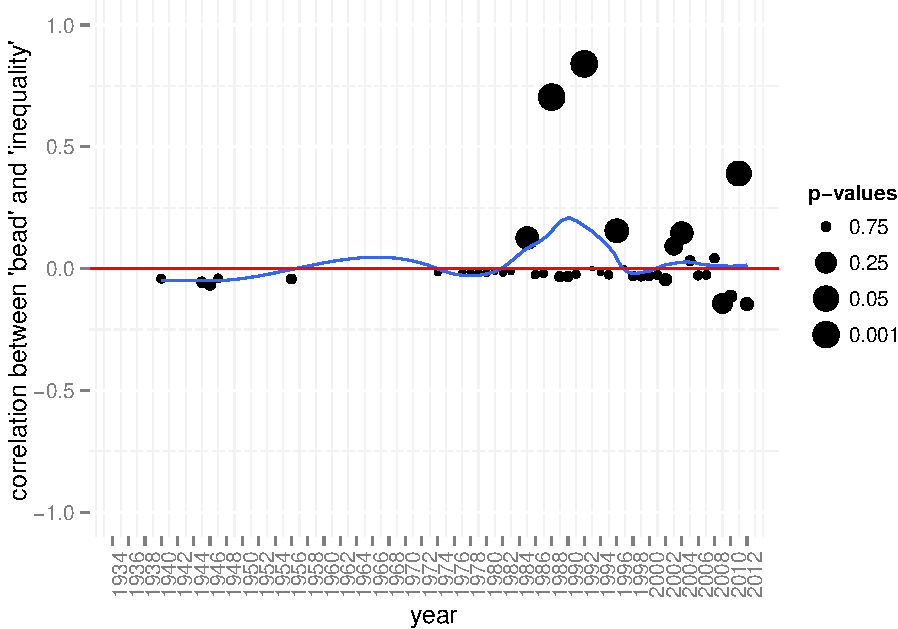
\includegraphics{509Assignment_files/figure-latex/onegram2-3} \end{CodeChunk}

The frequency of words containing ``inequality'' shows that the focus
changes with time. The focus of paper shift from population,
organization, and mound to ritual, power and pottery, which indicates
there is a trend of anthropological thinking from 2006. Besdies, The
term settlement could be observed in each period from 1996 until now,
and it becomes more popular over time.

\begin{CodeChunk}

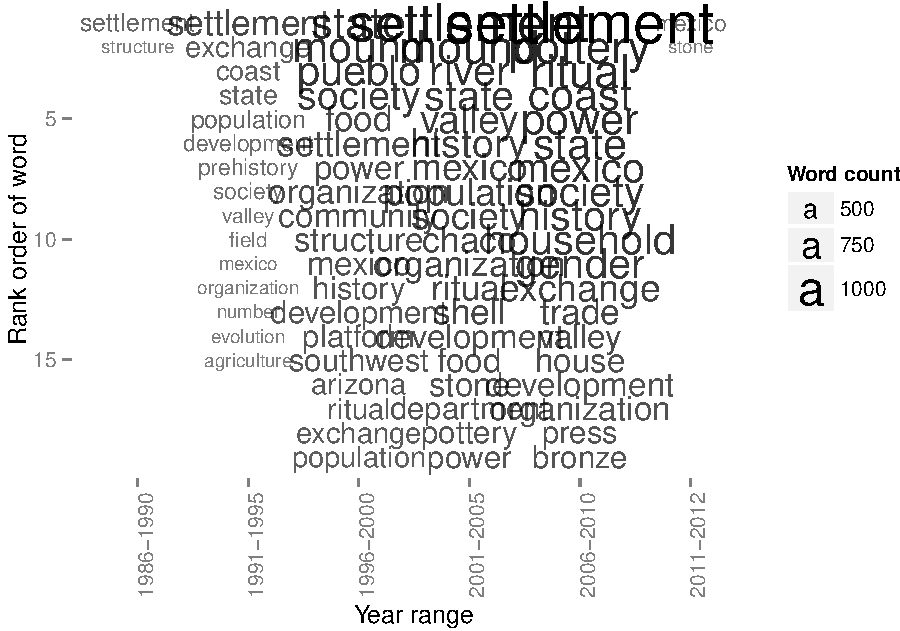
\includegraphics{509Assignment_files/figure-latex/onegram5-1} \end{CodeChunk}

TBA

\end{document}

